
\documentclass{article}
\usepackage[]{graphicx}\usepackage[]{color}
%% maxwidth is the original width if it is less than linewidth
%% otherwise use linewidth (to make sure the graphics do not exceed the margin)
\makeatletter
\def\maxwidth{ %
  \ifdim\Gin@nat@width>\linewidth
    \linewidth
  \else
    \Gin@nat@width
  \fi
}
\makeatother

\definecolor{fgcolor}{rgb}{0.345, 0.345, 0.345}
\newcommand{\hlnum}[1]{\textcolor[rgb]{0.686,0.059,0.569}{#1}}%
\newcommand{\hlstr}[1]{\textcolor[rgb]{0.192,0.494,0.8}{#1}}%
\newcommand{\hlcom}[1]{\textcolor[rgb]{0.678,0.584,0.686}{\textit{#1}}}%
\newcommand{\hlopt}[1]{\textcolor[rgb]{0,0,0}{#1}}%
\newcommand{\hlstd}[1]{\textcolor[rgb]{0.345,0.345,0.345}{#1}}%
\newcommand{\hlkwa}[1]{\textcolor[rgb]{0.161,0.373,0.58}{\textbf{#1}}}%
\newcommand{\hlkwb}[1]{\textcolor[rgb]{0.69,0.353,0.396}{#1}}%
\newcommand{\hlkwc}[1]{\textcolor[rgb]{0.333,0.667,0.333}{#1}}%
\newcommand{\hlkwd}[1]{\textcolor[rgb]{0.737,0.353,0.396}{\textbf{#1}}}%

\usepackage{framed}
\makeatletter
\newenvironment{kframe}{%
 \def\at@end@of@kframe{}%
 \ifinner\ifhmode%
  \def\at@end@of@kframe{\end{minipage}}%
  \begin{minipage}{\columnwidth}%
 \fi\fi%
 \def\FrameCommand##1{\hskip\@totalleftmargin \hskip-\fboxsep
 \colorbox{shadecolor}{##1}\hskip-\fboxsep
     % There is no \\@totalrightmargin, so:
     \hskip-\linewidth \hskip-\@totalleftmargin \hskip\columnwidth}%
 \MakeFramed {\advance\hsize-\width
   \@totalleftmargin\z@ \linewidth\hsize
   \@setminipage}}%
 {\par\unskip\endMakeFramed%
 \at@end@of@kframe}
\makeatother

\definecolor{shadecolor}{rgb}{.97, .97, .97}
\definecolor{messagecolor}{rgb}{0, 0, 0}
\definecolor{warningcolor}{rgb}{1, 0, 1}
\definecolor{errorcolor}{rgb}{1, 0, 0}
\newenvironment{knitrout}{}{} % an empty environment to be redefined in TeX

\usepackage{alltt}
\newcommand{\SweaveOpts}[1]{}  % do not interfere with LaTeX
\newcommand{\SweaveInput}[1]{} % because they are not real TeX commands
\newcommand{\Sexpr}[1]{}       % will only be parsed by R



% page dimensions
% \addtolength{\hoffset}{-1.5cm}
% \addtolength{\textwidth}{3cm}
% \addtolength{\voffset}{-1cm}
% \addtolength{\textheight}{2cm}
\usepackage[margin=1in]{geometry}
\usepackage{xspace}
\usepackage{url}
\usepackage{mdwlist}
%\usepackage{breakurl}
\usepackage[authoryear]{natbib}
\bibliographystyle{abbrvnat-apa}
% \usepackage[unicode=true,pdfusetitle,
%  bookmarks=true,bookmarksnumbered=true,bookmarksopen=true,bookmarksopenlevel=3,
%  breaklinks=true,pdfborder={0 0 1},backref=false,colorlinks=false]
%  {hyperref}

%% Define needed commands here; these should go in a style file
%% or be \input{}

% Cross-references
\newcommand{\eqref}[1]{(\ref{#1})}
\newcommand{\chref}[1]{Chapter~\ref{#1}}
\newcommand{\secref}[1]{Section~\ref{#1}}
\newcommand{\figref}[1]{Figure~\ref{#1}}
\newcommand{\tabref}[1]{Table~\ref{#1}}

% float parameters
\renewcommand{\textfraction}{0.05}
\renewcommand{\topfraction}{0.8}
\renewcommand{\bottomfraction}{0.8}
\renewcommand{\floatpagefraction}{0.75}


% writing about R stuff; these can be modified to add indexing, etc.
\newcommand{\var}[1]{\textit{\texttt{#1}}}
\newcommand{\data}[1]{\texttt{#1}}
\newcommand{\class}[1]{\textsf{"#1"}}
% may need a more robust version of \code to handle special chars
% this doesn't quite handle it.
\makeatletter
\newcommand\code{\bgroup\@makeother\_\@makeother\~\@makeother\$\@codex}
\def\@codex#1{{\normalfont\ttfamily\hyphenchar\font=-1 #1}\egroup}
\makeatother
%\newcommand{\code}[1]{\texttt{#1}}
\newcommand{\func}[1]{\code{#1()}}
\let\proglang=\textsf
\newcommand{\R}{\proglang{R}\xspace}

% should redefine \pkg to also cite the package, but this requires
% an extra, optional argument.
%\newcommand{\pkg}[1]{{\normalfont\fontseries{b}\selectfont #1}}
\newcommand{\pkg}[1]{\textsf{#1}\nocite{R-#1}}
\newcommand{\Rpackage}[1]{\pkg{#1} package}

\newcommand{\glossterm}[1]{\textit{\textbf{#1}}}

% simplified Example environment
\newenvironment{Example}[2][unnamed-example]%
  {\medskip\noindent\textbf{\textsf{Example:}}
   \textbf{#2}\hfill [#1]\par\smallskip
  }
  {\hfill $\triangle$}
  
% stop overfull hbox whining
\hfuzz=12pt


% enable TeX lookup from localtexmf
% following ideas from http://texblog.org/2013/08/20/rknitr-automatic-bibliography-generation-with-biblatex-in-rstudio/




\begin{document}
% !Rnw weave = knitr





\section*{Classification and regression trees}

Recursive partitioning methods provide an alternative to (generalized) linear
models for categorical responses, particularly when there are numerous
potential predictors and/or there are important interactions among predictors.

These methods attempt to define a set of rules to classify observations into
mutually exclusive subsets based on combinations of the explanatory variables.
In contrast to linear models, where it is necessary to \emph{explicitly}
specify the form of all model terms, recursive partitioning methods
tend to work well when there are important non-linearities or interactions
in the data.  

We illustrate some of the ideas behind these methods with
the \Rpackage{rpart}, for fitting recursive partitioning trees,%
\footnote{\pkg{rpart} is an \R implementation of the CART
(\emph{Classification and Regression Trees})
book and software of \citet{Breiman-etal:1984}}
and the
\Rpackage{party}, which embeds tree-structured models within a general
framework of conditional inference procedures.  

For a \emph{binary} response variable, \func{rpart} fits a tree to predict the
outcome using a two-stage procedure:  
\begin{enumerate*}
  \item First, the observations are partitioned
into prediction classes (e.g., ``lived'', ``died'') by using univariate, binary splits
on the available predictors in a recursive way.  

  \item A second stage is then applied to evaluate the resulting binary tree, using some
methods of testing and cross-validation to prune the tree according to some
criterion.
\end{enumerate*}

% This text from the rpart vignette -- revise & cite
In the first stage, tree is built by the following process: 
\begin{itemize*}
  \item First the single variable is found which best splits the data into two groups.
  \item The data is separated, and then this process is applied separately to each sub-group
  \item These steps are applied recursively until the sub-groups either reach a minimum size or until no improvement can be
made.
\end{itemize*}

In practical use, there are many options and parameters to control the details of the analysis, such as 
\begin{itemize*}
  \item the minimum number of observations in a node for a split to be made (\code{minsplit}), 
  \item a complexity parameter (\code{cp}) measuring the ``cost'' of adding another variable to the model, 
  \item the maximum depth (\code{maxdepth}) of any node in the final tree, and so forth. 
\end{itemize*}
These can be set in the call to \func{rpart}, using arguments described in \code{help(rpart.control)}. 

\begin{Example}[titanic-tree]{Survival on the \emph{Titanic}: Recursive partitioning trees}

This example uses the \data{Titanicp} from \pkg{vcdExtra} data we have examined in other examples in the book.
We first fit an \func{rpart} tree to predict survival using only age and passenger class.
The \Rpackage{rpart.plot} can plot such trees, and provides numerous options to 
control the details of what is plotted for each node.  
The focus here is on visualization methods for interpreting the results.

\begin{knitrout}
\definecolor{shadecolor}{rgb}{0.969, 0.969, 0.969}\color{fgcolor}\begin{kframe}
\begin{alltt}
\hlcom{# fit a simple tree, using only pclass and age}
\hlkwd{library}\hlstd{(rpart)}
\hlkwd{library}\hlstd{(rpart.plot)}
\hlkwd{data}\hlstd{(Titanicp,} \hlkwc{package}\hlstd{=}\hlstr{"vcdExtra"}\hlstd{)}
\hlstd{rp0} \hlkwb{<-} \hlkwd{rpart}\hlstd{(survived} \hlopt{~} \hlstd{pclass} \hlopt{+} \hlstd{age,} \hlkwc{data}\hlstd{=Titanicp)}
\hlkwd{rpart.plot}\hlstd{(rp0,} \hlkwc{type}\hlstd{=}\hlnum{0}\hlstd{,} \hlkwc{extra}\hlstd{=}\hlnum{2}\hlstd{,} \hlkwc{cex}\hlstd{=}\hlnum{1.5}\hlstd{)}
\end{alltt}
\end{kframe}\begin{figure}[hbt!]

{\centering 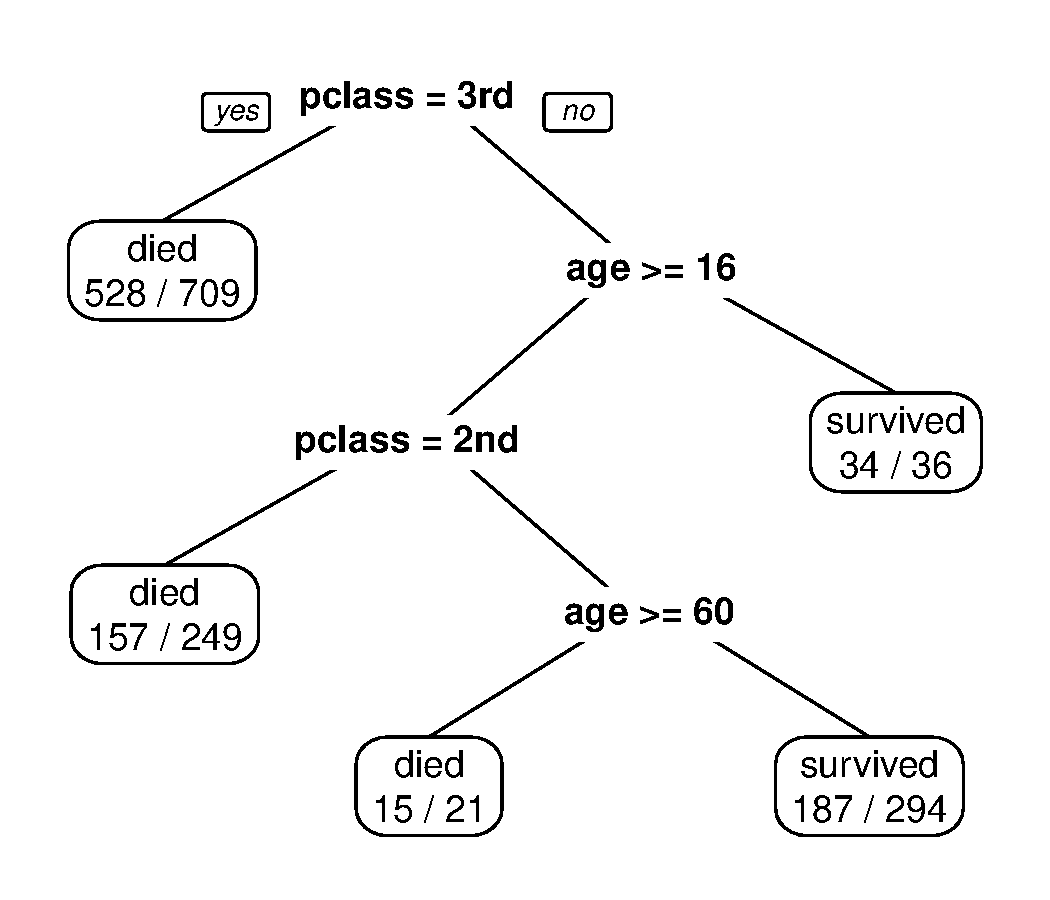
\includegraphics[width=0.55\linewidth]{figure/rp0-1} 

}

\caption[Classification tree for passengers on the \emph{Titanic}, using \var{pclass} and \var{age}]{Classification tree for passengers on the \emph{Titanic}, using \var{pclass} and \var{age}.}\label{fig:rp0}
\end{figure}


\end{knitrout}

The basic tree shown
in \figref{fig:rp0} displays the levels of the variables used for
classification at each node. 
The tree is read as follows:
Each non-terminal (unboxed) node represents a decision based on one variable,
where the left branch corresponds to \code{TRUE} and the right branch \code{FALSE}.

For example, the first split separates 3$^{rd}$
class passengers from the rest, and the next split on the right is between those older
than 16, in class 1 and 2.  
The terminal nodes (leaves) with ovals indicate the
prediction for that partition and number who lived or died out of the
total in that subgroup. For example, those with \code{age<16} in class
1 and 2 are predicted to have survived and 34 out of 36 did so.
The bottom left leaf represents 1$^{st}$ class passengers with \code{age<60},
where 187 out of 294 survived.

Printing the resulting \class{rpart} object
(\code{rp0}, here) gives a text representation of the model.
The legend indicates that each line contains the node number,
splitting variable and value (\code{split}), 
the number (\code{n}) of observations at that node,
the number (\code{loss}) of observations incorrectly classified,
the predicted classification at that node (\code{yval}),
and the probabilities of the response classes at that node
(\code{yprob}).  Leaf nodes are indicated by the trailing \code{"*"}.
\begin{knitrout}
\definecolor{shadecolor}{rgb}{0.969, 0.969, 0.969}\color{fgcolor}\begin{kframe}
\begin{alltt}
\hlstd{rp0}
\end{alltt}
\begin{verbatim}
## n= 1309 
## 
## node), split, n, loss, yval, (yprob)
##       * denotes terminal node
## 
##  1) root 1309 500 died (0.61802903 0.38197097)  
##    2) pclass=3rd 709 181 died (0.74471086 0.25528914) *
##    3) pclass=1st,2nd 600 281 survived (0.46833333 0.53166667)  
##      6) age>=15.5 564 279 survived (0.49468085 0.50531915)  
##       12) pclass=2nd 249  92 died (0.63052209 0.36947791) *
##       13) pclass=1st 315 122 survived (0.38730159 0.61269841)  
##         26) age>=60.5 21   6 died (0.71428571 0.28571429) *
##         27) age< 60.5 294 107 survived (0.36394558 0.63605442) *
##      7) age< 15.5 36   2 survived (0.05555556 0.94444444) *
\end{verbatim}
\end{kframe}
\end{knitrout}
The information here is a faithful textual representation of the
tree, but much harder to read than the visual representation in
\figref{fig:rp0}.


Any such recursive partitioning tree can be visualized instead by a
\glossterm{treemap} or partition map, which divides a unit rectangle
into regions based on the variable splits.%
\footnote{
The idea for this plot comes from Varian (2013),
\url{http://people.ischool.berkeley.edu/~hal/Papers/2013/ml.pdf}.
}
This is easiest to show
for two variables, where we can also plot the individual observations.
\figref{fig:partition-map1} is the treemap representation of the
tree in \figref{fig:rp0}.  The \R code uses basic \func{plot} facilities
and isn't shown here.

\begin{knitrout}
\definecolor{shadecolor}{rgb}{0.969, 0.969, 0.969}\color{fgcolor}\begin{figure}[hbt!]

{\centering 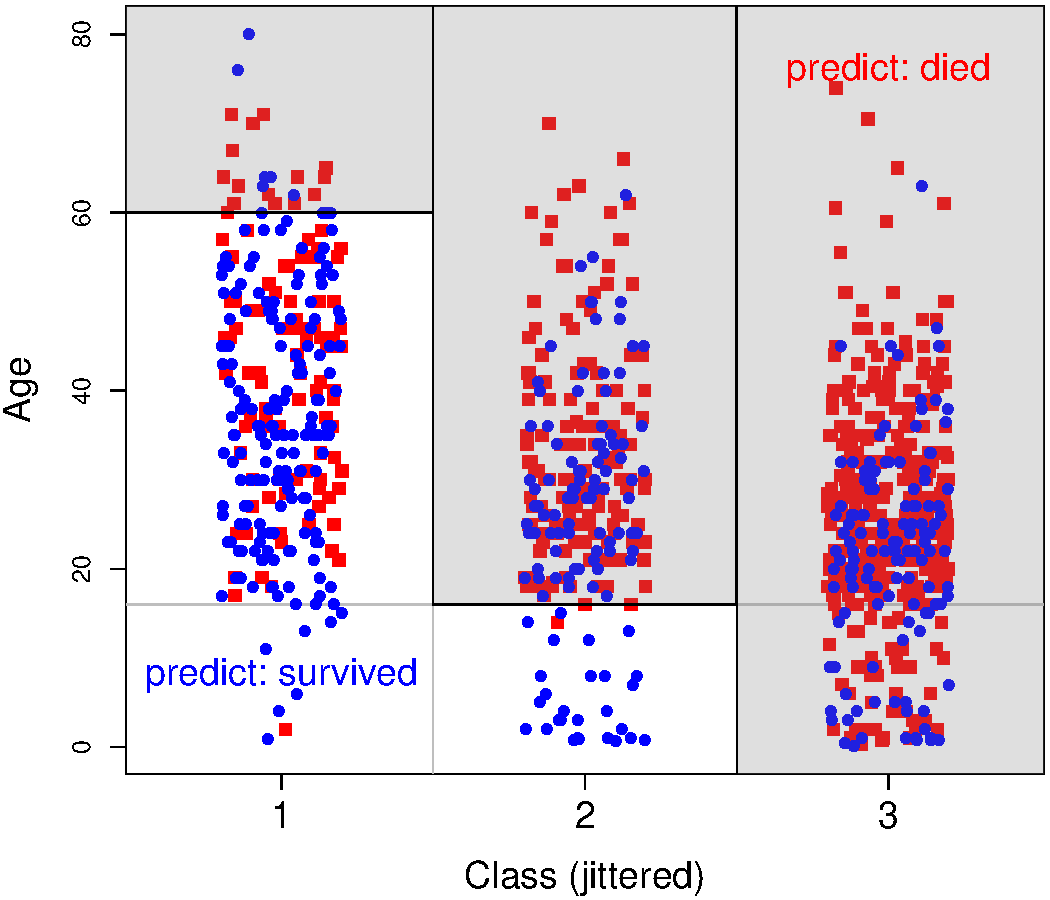
\includegraphics[width=0.7\linewidth]{figure/partition-map1-1} 

}

\caption[]{Partition map for the tree in \figref{fig:rp0}.  Those in the shaded region are predicted to have died; observations are shown by red circles (died) and blue squares (survived)}\label{fig:partition-map1}
\end{figure}


\end{knitrout}

A similar treemap can be produced using the \Rpackage{plotmo}.  This has many
options for plotting a model response in models with one or two predictors.
In the call below, \code{type2="image"} says to plot the two-way effect
of \code{pclass:age} as a shaded image.

\begin{knitrout}
\definecolor{shadecolor}{rgb}{0.969, 0.969, 0.969}\color{fgcolor}\begin{kframe}
\begin{alltt}
\hlkwd{library}\hlstd{(plotmo)}
\hlkwd{plotmo}\hlstd{(rp0,} \hlkwc{nresponse}\hlstd{=}\hlstr{"survived"}\hlstd{,} \hlkwc{degree1}\hlstd{=}\hlnum{0}\hlstd{,} \hlkwc{type2}\hlstd{=}\hlstr{"image"}\hlstd{,}
  \hlkwc{col.image}\hlstd{=}\hlkwd{gray}\hlstd{(}\hlkwd{seq}\hlstd{(}\hlnum{.6}\hlstd{,} \hlnum{1}\hlstd{,}\hlnum{.05}\hlstd{)),}
  \hlkwc{col.response}\hlstd{=}\hlkwd{ifelse}\hlstd{(Titanicp}\hlopt{$}\hlstd{survived}\hlopt{==}\hlstr{"died"}\hlstd{,} \hlstr{"red"}\hlstd{,} \hlstr{"blue"}\hlstd{),}
  \hlkwc{pch}\hlstd{=}\hlkwd{ifelse}\hlstd{(Titanicp}\hlopt{$}\hlstd{survived}\hlopt{==}\hlstr{"died"}\hlstd{,} \hlnum{15}\hlstd{,} \hlnum{16}\hlstd{))}
\end{alltt}
\end{kframe}\begin{figure}[hbt!]

{\centering 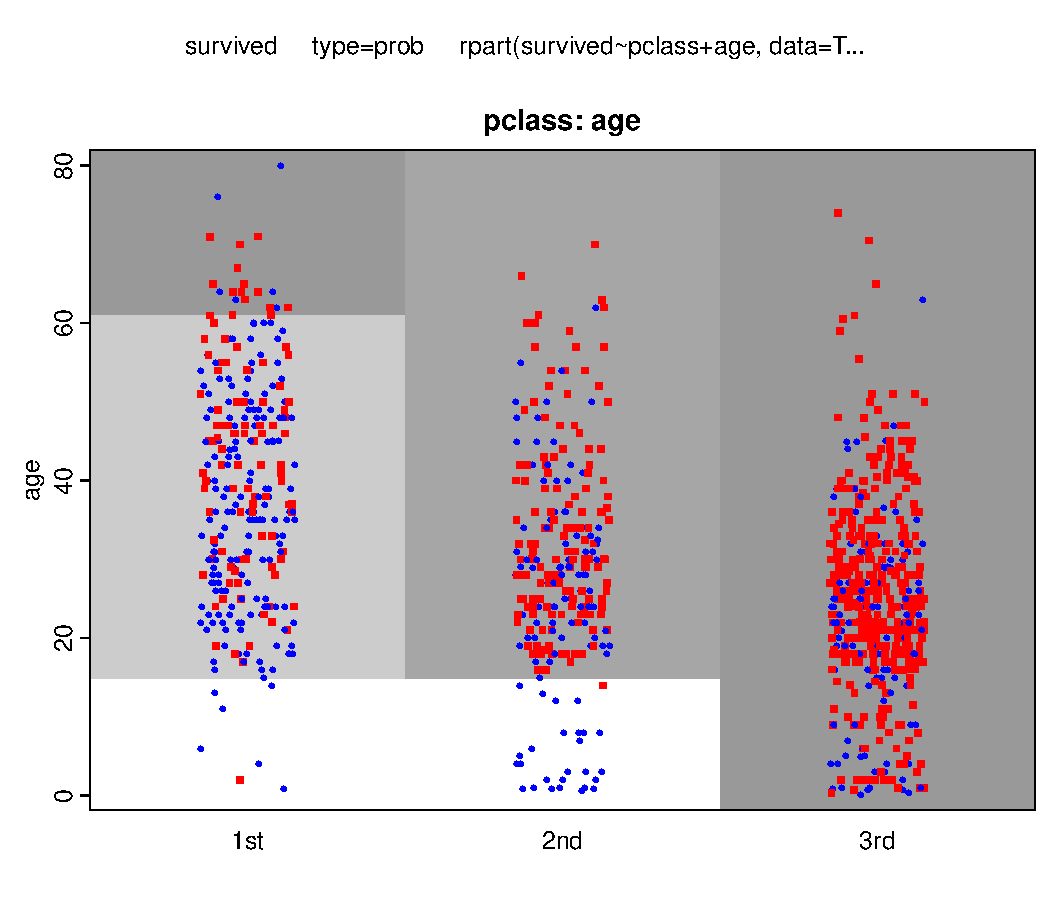
\includegraphics[width=0.7\linewidth]{figure/rp-plotmo1-1} 

}

\caption[]{\func{plotmo} plot for the tree in \figref{fig:rp0}. Shading level is proportional to the predicted probability of survival.}\label{fig:rp-plotmo1}
\end{figure}


\end{knitrout}

\func{plotmo} is much more general than this, and can handle models
fit with \func{lm}, \func{glm}, \func{gam}, \func{lda} and others
in addition to \func{rpart}.
Similar to an effects plot, it allows plotting the response
in a model as one or two predictors are varied, holding all other predictors
constant (continuous variables at their medians;
factors, at their first level, by default). 
By default, the function plots the response for all main effects (\code{degree1=})
and all two-way effects (\code{degree2=}) in a single multi-panel plot.
Here we produce them separately, in order to lay them out side-by-side.
\begin{knitrout}
\definecolor{shadecolor}{rgb}{0.969, 0.969, 0.969}\color{fgcolor}\begin{kframe}
\begin{alltt}
\hlcom{# one-way plots}
\hlkwd{plotmo}\hlstd{(rp0,} \hlkwc{nresponse}\hlstd{=}\hlstr{"survived"}\hlstd{,} \hlkwc{degree1}\hlstd{=}\hlnum{1}\hlstd{,} \hlkwc{degree2}\hlstd{=}\hlnum{0}\hlstd{,} \hlkwc{trace}\hlstd{=}\hlopt{-}\hlnum{1}\hlstd{,} \hlkwc{do.par}\hlstd{=}\hlnum{FALSE}\hlstd{)}
\hlkwd{plotmo}\hlstd{(rp0,} \hlkwc{nresponse}\hlstd{=}\hlstr{"survived"}\hlstd{,} \hlkwc{degree1}\hlstd{=}\hlnum{2}\hlstd{,} \hlkwc{degree2}\hlstd{=}\hlnum{0}\hlstd{,} \hlkwc{trace}\hlstd{=}\hlopt{-}\hlnum{1}\hlstd{,} \hlkwc{do.par}\hlstd{=}\hlnum{FALSE}\hlstd{)}
\hlcom{# two-way, 3D persp plot}
\hlkwd{plotmo}\hlstd{(rp0,} \hlkwc{nresponse}\hlstd{=}\hlstr{"survived"}\hlstd{,} \hlkwc{degree1}\hlstd{=}\hlnum{0}\hlstd{,} \hlkwc{trace}\hlstd{=}\hlopt{-}\hlnum{1}\hlstd{)}
\end{alltt}
\end{kframe}\begin{figure}[hbt!]

{\centering 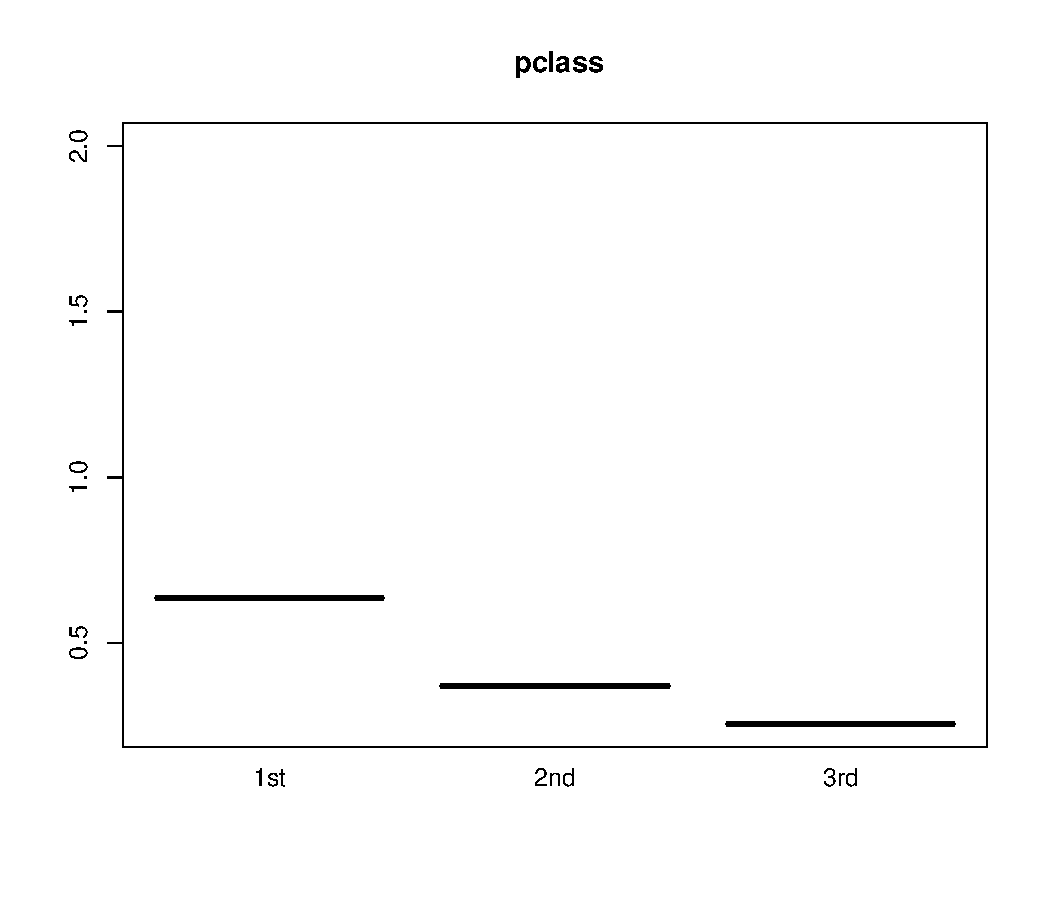
\includegraphics[width=0.32\linewidth]{figure/rp-plotmo2-1} 
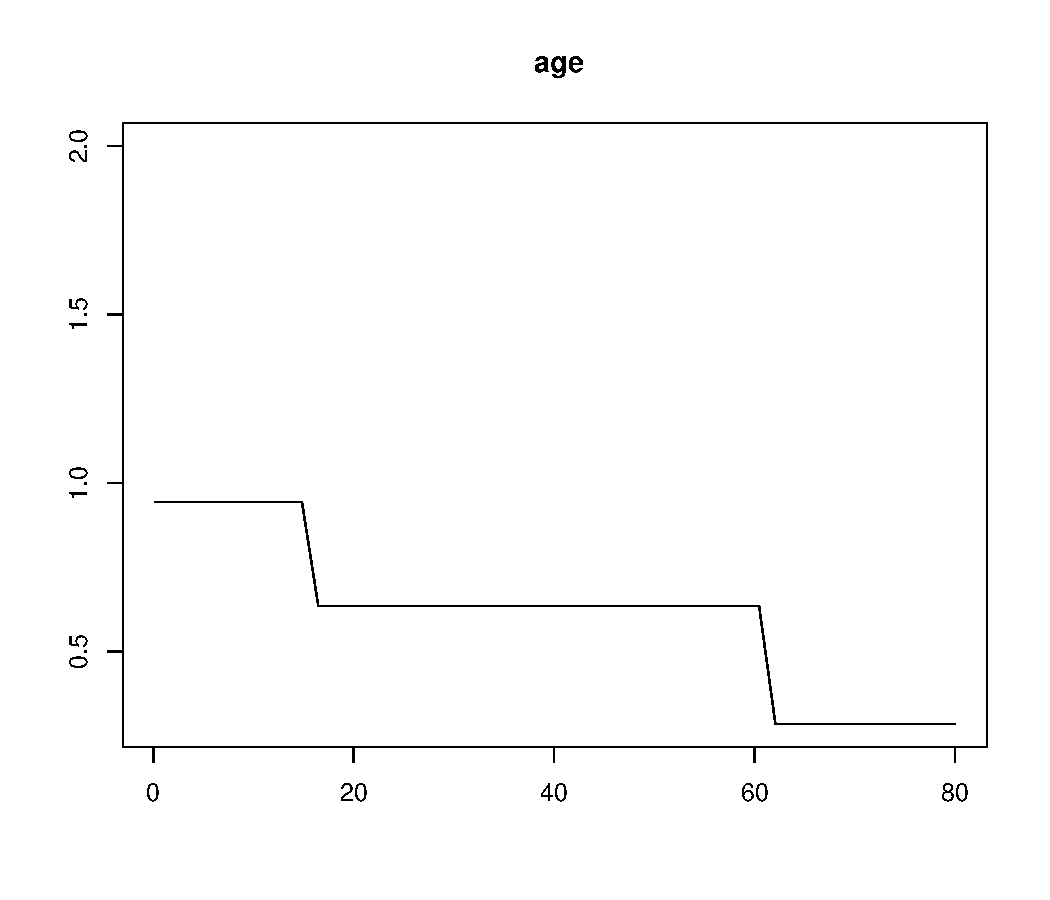
\includegraphics[width=0.32\linewidth]{figure/rp-plotmo2-2} 
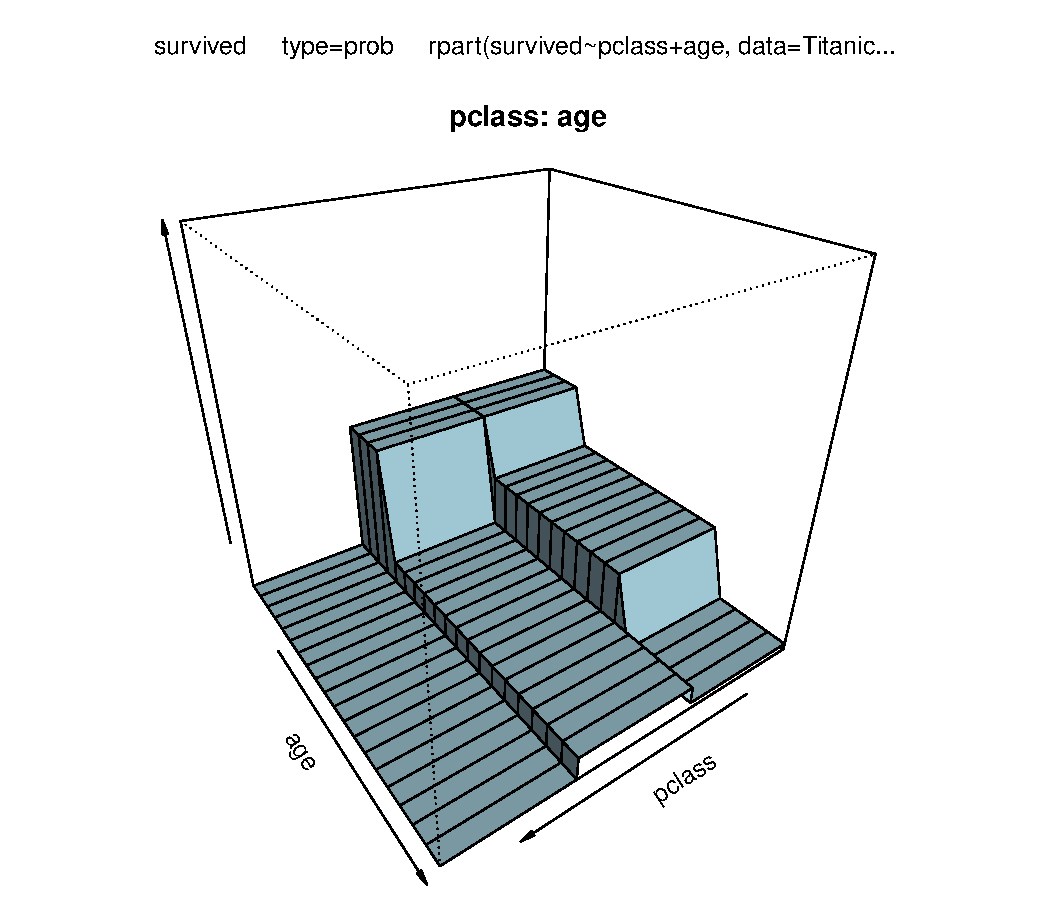
\includegraphics[width=0.32\linewidth]{figure/rp-plotmo2-3} 

}

\caption[Other \func{plotmo} plots]{Other \func{plotmo} plots: one-way and two-way effects}\label{fig:rp-plotmo2}
\end{figure}


\end{knitrout}
Note that the image plot in \figref{fig:rp-plotmo1} is a view from above of the
3D right panel in \figref{fig:rp-plotmo2}. Some care is needed in interpreting the
one-way plots When there are factors in the model, because the default
``constant'' value is the first level of a factor.
For example, the middle plot shows the predictions for \var{age} for those
in 1$^{st}$ class.%  
\footnote{
Effect plots, in the \Rpackage{effects} provide a more general way to average
over factors, but are not available for \class{rpart} models
}
This can be seen in as the profile of the right-most 
step function in the 3D image in the right panels \figref{fig:rp-plotmo1}.

\subsection*{Pruning}
At each split, \func{rpart} calculates a number of statistics, including
a complexity parameter (\code{cp}) and measures of the error (\code{error}) 
in classification,
as well as the mean (\code{xerror}) and standard deviation (\code{xstd})
of the errors in the cross-validated prediction.
This information can be printed using \func{printcp} and plotted with \func{printcp},
as shown in \figref{fig:plotcp-rp0}.
\begin{knitrout}
\definecolor{shadecolor}{rgb}{0.969, 0.969, 0.969}\color{fgcolor}\begin{kframe}
\begin{alltt}
\hlkwd{printcp}\hlstd{(rp0)}
\end{alltt}
\begin{verbatim}
## 
## Classification tree:
## rpart(formula = survived ~ pclass + age, data = Titanicp)
## 
## Variables actually used in tree construction:
## [1] age    pclass
## 
## Root node error: 500/1309 = 0.38197
## 
## n= 1309 
## 
##      CP nsplit rel error xerror     xstd
## 1 0.076      0     1.000  1.000 0.035158
## 2 0.065      1     0.924  0.994 0.035117
## 3 0.018      3     0.794  0.818 0.033538
## 4 0.010      4     0.776  0.792 0.033239
\end{verbatim}
\end{kframe}
\end{knitrout}
\begin{knitrout}
\definecolor{shadecolor}{rgb}{0.969, 0.969, 0.969}\color{fgcolor}\begin{kframe}
\begin{alltt}
\hlkwd{plotcp}\hlstd{(rp0,} \hlkwc{lty}\hlstd{=}\hlnum{2}\hlstd{,} \hlkwc{col}\hlstd{=}\hlstr{"red"}\hlstd{,} \hlkwc{lwd}\hlstd{=}\hlnum{2}\hlstd{)}
\end{alltt}
\end{kframe}\begin{figure}[hbt!]

{\centering 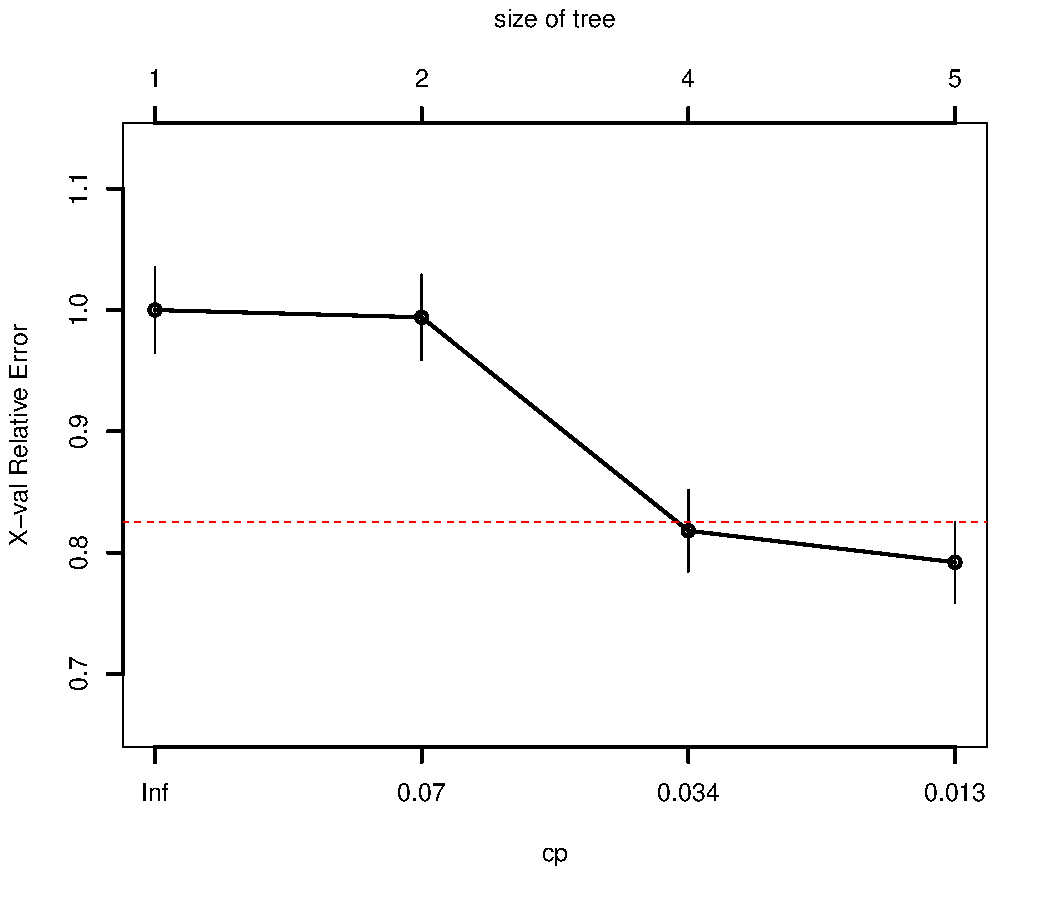
\includegraphics[width=0.6\linewidth]{figure/plotcp-rp0-1} 

}

\caption[Plot of complexity and error statistics]{Plot of complexity and error statistics. The dashed horizontal line is drawn 1 SE above the minimum of the curve.}\label{fig:plotcp-rp0}
\end{figure}


\end{knitrout}

There is not really any need to prune this small tree, but for illustration,
we can use this information to prune the tree, and then plot the pruned result,
this time with additional options (\figref{fig:rp0-pruned}).
The option \code{extra=2} shows the classification of the observations
that reach each node and \code{box.col} allows the node ovals to be
colored.

\begin{knitrout}
\definecolor{shadecolor}{rgb}{0.969, 0.969, 0.969}\color{fgcolor}\begin{kframe}
\begin{alltt}
\hlstd{rp0.pruned} \hlkwb{<-} \hlkwd{prune}\hlstd{(rp0,} \hlkwc{cp}\hlstd{=}\hlnum{.05}\hlstd{)}
\hlkwd{rpart.plot}\hlstd{(rp0.pruned,} \hlkwc{type}\hlstd{=}\hlnum{0}\hlstd{,} \hlkwc{extra}\hlstd{=}\hlnum{2}\hlstd{,} \hlkwc{cex}\hlstd{=}\hlnum{1.5}\hlstd{,}
           \hlkwc{under}\hlstd{=}\hlnum{TRUE}\hlstd{,} \hlkwc{box.col}\hlstd{=}\hlkwd{c}\hlstd{(}\hlstr{"pink"}\hlstd{,} \hlstr{"lightblue"}\hlstd{)[rp0.pruned}\hlopt{$}\hlstd{frame}\hlopt{$}\hlstd{yval])}
\end{alltt}
\end{kframe}\begin{figure}[hbt!]

{\centering 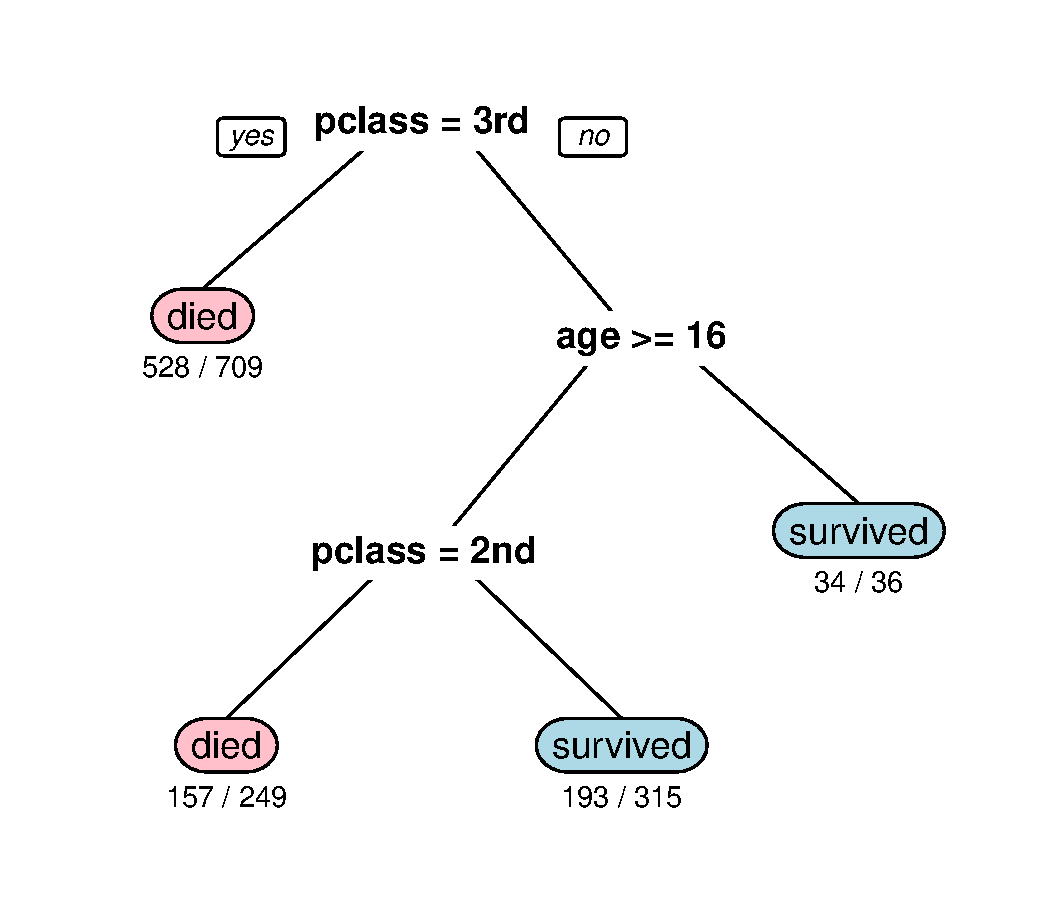
\includegraphics[width=0.6\linewidth]{figure/rp0-pruned-1} 

}

\caption[Classification tree for passengers on the Titanic, pruned]{Classification tree for passengers on the Titanic, pruned}\label{fig:rp0-pruned}
\end{figure}


\end{knitrout}

\subsection*{Larger models}
Continuing, we now include \var{sex} and \var{sibsp} 
(number of siblings and parents)
among the predictors.  
\begin{knitrout}
\definecolor{shadecolor}{rgb}{0.969, 0.969, 0.969}\color{fgcolor}\begin{kframe}
\begin{alltt}
\hlstd{rp1} \hlkwb{=} \hlkwd{rpart}\hlstd{(survived} \hlopt{~} \hlstd{pclass} \hlopt{+} \hlstd{sex} \hlopt{+} \hlstd{age} \hlopt{+} \hlstd{sibsp,} \hlkwc{data}\hlstd{=Titanicp)}
\end{alltt}
\end{kframe}
\end{knitrout}
In the table of complexity parameters, there is no evidence of a need to prune this
tree.
\begin{knitrout}
\definecolor{shadecolor}{rgb}{0.969, 0.969, 0.969}\color{fgcolor}\begin{kframe}
\begin{alltt}
\hlkwd{printcp}\hlstd{(rp1)}
\end{alltt}
\begin{verbatim}
## 
## Classification tree:
## rpart(formula = survived ~ pclass + sex + age + sibsp, data = Titanicp)
## 
## Variables actually used in tree construction:
## [1] age    pclass sex    sibsp 
## 
## Root node error: 500/1309 = 0.38197
## 
## n= 1309 
## 
##      CP nsplit rel error xerror     xstd
## 1 0.424      0     1.000  1.000 0.035158
## 2 0.021      1     0.576  0.576 0.029976
## 3 0.015      3     0.534  0.596 0.030342
## 4 0.014      5     0.504  0.580 0.030050
## 5 0.012      7     0.476  0.540 0.029279
## 6 0.010      8     0.464  0.522 0.028911
\end{verbatim}
\end{kframe}
\end{knitrout}

We plot the tree, using the \func{rpart.plot} again, giving \figref{fig:rp1}.

\begin{knitrout}
\definecolor{shadecolor}{rgb}{0.969, 0.969, 0.969}\color{fgcolor}\begin{kframe}
\begin{alltt}
\hlkwd{rpart.plot}\hlstd{(rp1,} \hlkwc{type}\hlstd{=}\hlnum{4}\hlstd{,} \hlkwc{extra}\hlstd{=}\hlnum{2}\hlstd{,} \hlkwc{faclen}\hlstd{=}\hlnum{0}\hlstd{,} \hlkwc{under}\hlstd{=}\hlnum{TRUE}\hlstd{,} \hlkwc{cex}\hlstd{=}\hlnum{1.1}\hlstd{,}
  \hlkwc{box.col}\hlstd{=}\hlkwd{c}\hlstd{(}\hlstr{"pink"}\hlstd{,} \hlstr{"lightblue"}\hlstd{)[rp1}\hlopt{$}\hlstd{frame}\hlopt{$}\hlstd{yval])}
\end{alltt}
\end{kframe}\begin{figure}[hbt!]

{\centering 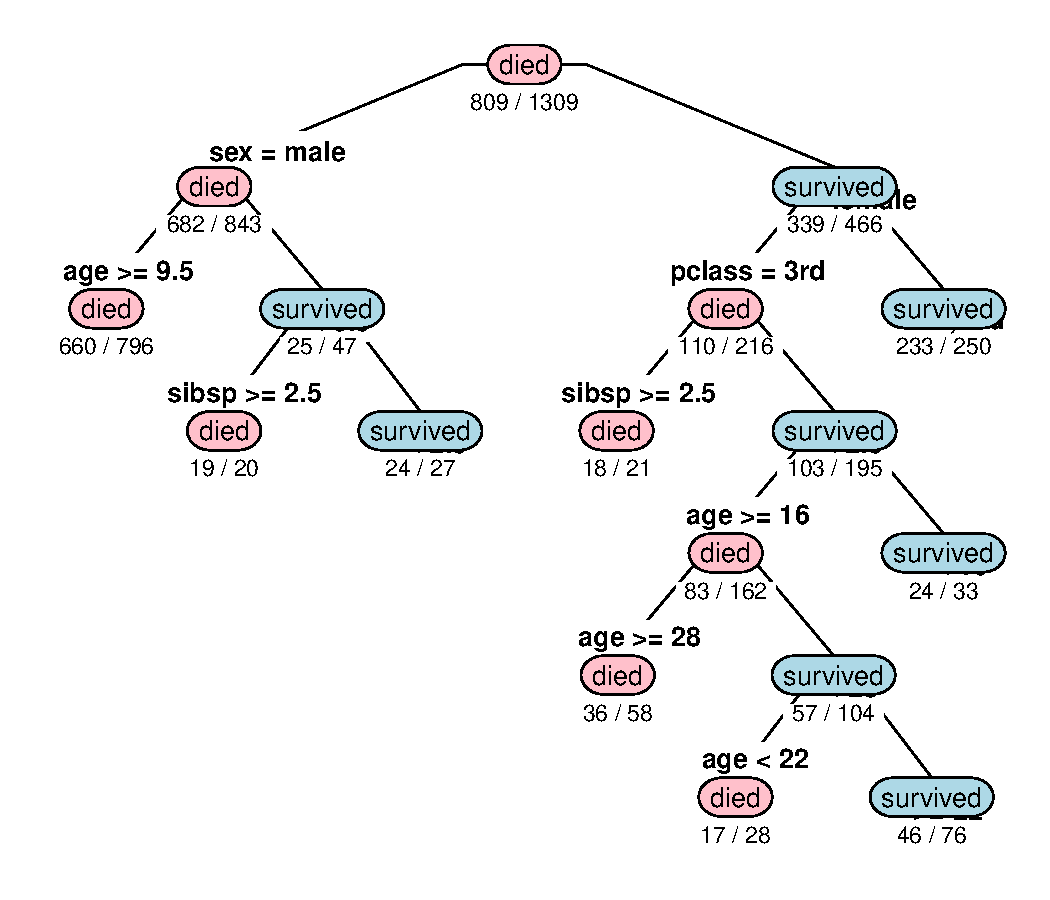
\includegraphics[width=.7\linewidth]{figure/rp1-1} 

}

\caption[Plot of the extended \func{rpart} tree for four predictors]{Plot of the extended \func{rpart} tree for four predictors}\label{fig:rp1}
\end{figure}


\end{knitrout}
\var{sex} is now the primary splitting variables.  Interestingly, among
male passengers, with an overall low survival rate,
survival is next predicted by \var{age} and then family size
(\var{sibsp});  passenger class doesn't matter here.
Among female passengers, those in class 1 and 2 are predicted to survive,
regardless of other predictors, while predictions for those in 3$^{rd}$
class with large families (\code{sibsp} $ge$ 2.5) are gloomy (``died''),
but among those in smaller predicted outcome depends on age.

This example nicely illustrates the difference between tree-based models
and standard (generalized) linear models for a binary response.
Recursive partitioning methods provide a nested set of decision rules 
depending on various subsets of the predictor variable values.
There is no need, within these methods to ask or test whether 
the predictor effects are linear or nonlinear, nor is there an need
to model interactions among predictors explicitly (which ones?),
because the recursive partioning of the observations automatically
takes care of combinations of predictors that appear in the various
branches.


\end{Example}

\begin{Example}[titanic-ctree]{Conditional inference trees}

\func{rpart} classification trees use internal cross-validation
to balance model complexity against goodness of fit, particularly
for out-of-sample prediction. The complexity parameter (\code{cp})
mentioned earlier imposes a cost for having many branches,
in a way analogous to other shrinkage methods (lasso, ridge regression, etc.)
and statistics (AIC, BIC).

However, these methods are subject to overfitting (hence, the need for
pruning) and have an ad hoc flavor, since they don't use any 
statistical notion to distinguish significant from insignificant
improvements with additional splits.
The conditional inference framework embodied in the \Rpackage{party}
solves these problems by embedding recursive partioning methods within
a general theory of permutation tests stemming from
\citet{StrasserWeber:1999}
%Strasser and Weber (1999). 

Essentially, a linear statistic is calculated to test the hypothesis
of independence between the response, $Y$, and each predictor.  A $p$-value
for that test can be calculated with reference to the permutation
distribution over all permutations of $Y$. The procedure stops if
none of the predictors allows this null hypothesis to be rejected;
otherwise the variable with the strongest association to $Y$ is
selected for the next split.


Here we fit a conditional inference tree, using \func{ctree} from the
\Rpackage{party} and the predictors \var{pclass}, \var{sex} and \var{age}.
\begin{knitrout}
\definecolor{shadecolor}{rgb}{0.969, 0.969, 0.969}\color{fgcolor}\begin{kframe}
\begin{alltt}
\hlkwd{library}\hlstd{(party)}
\hlstd{titanic.ctree} \hlkwb{=} \hlkwd{ctree}\hlstd{(survived} \hlopt{~} \hlstd{pclass} \hlopt{+} \hlstd{sex} \hlopt{+} \hlstd{age,} \hlkwc{data}\hlstd{=Titanicp)}
\hlstd{titanic.ctree}
\end{alltt}
\begin{verbatim}
## 
## 	 Conditional inference tree with 8 terminal nodes
## 
## Response:  survived 
## Inputs:  pclass, sex, age 
## Number of observations:  1309 
## 
## 1) sex == {male}; criterion = 1, statistic = 365.607
##   2) pclass == {1st}; criterion = 1, statistic = 32.994
##     3) age <= 54; criterion = 0.992, statistic = 9.079
##       4)*  weights = 151 
##     3) age > 54
##       5)*  weights = 28 
##   2) pclass == {2nd, 3rd}
##     6) age <= 9; criterion = 1, statistic = 25.406
##       7) pclass == {2nd}; criterion = 0.998, statistic = 12.103
##         8)*  weights = 11 
##       7) pclass == {3rd}
##         9)*  weights = 29 
##     6) age > 9
##       10)*  weights = 624 
## 1) sex == {female}
##   11) pclass == {1st, 2nd}; criterion = 1, statistic = 115.454
##     12) pclass == {2nd}; criterion = 0.956, statistic = 5.911
##       13)*  weights = 106 
##     12) pclass == {1st}
##       14)*  weights = 144 
##   11) pclass == {3rd}
##     15)*  weights = 216
\end{verbatim}
\end{kframe}
\end{knitrout}
The \func{plot} method for \class{ctree} objects is very flexible.
The following call produces \figref{fig:titanic-ctree}.
Each non-terminal node is labeled with the $p$-value for that split,
and the barplot for each leaf node shows the proportion of survivors on that branch.
The arguments to \func{plot.ctree} can include panel functions
used to plot the interior nodes (\code{inner\_panel=node\_inner} here)
and leaf nodes (\code{terminal\_panel=node\_barplot} here).
\begin{knitrout}
\definecolor{shadecolor}{rgb}{0.969, 0.969, 0.969}\color{fgcolor}\begin{kframe}
\begin{alltt}
\hlkwd{plot}\hlstd{(titanic.ctree,}
  \hlkwc{tp_args} \hlstd{=} \hlkwd{list}\hlstd{(}\hlkwc{fill} \hlstd{=} \hlkwd{c}\hlstd{(}\hlstr{"blue"}\hlstd{,} \hlstr{"lightgray"}\hlstd{)),}
  \hlkwc{ip_args} \hlstd{=} \hlkwd{list}\hlstd{(}\hlkwc{fill} \hlstd{=} \hlkwd{c}\hlstd{(}\hlstr{"lightgreen"}\hlstd{))}
        \hlstd{)}
\end{alltt}
\end{kframe}\begin{figure}[hbt!]

{\centering 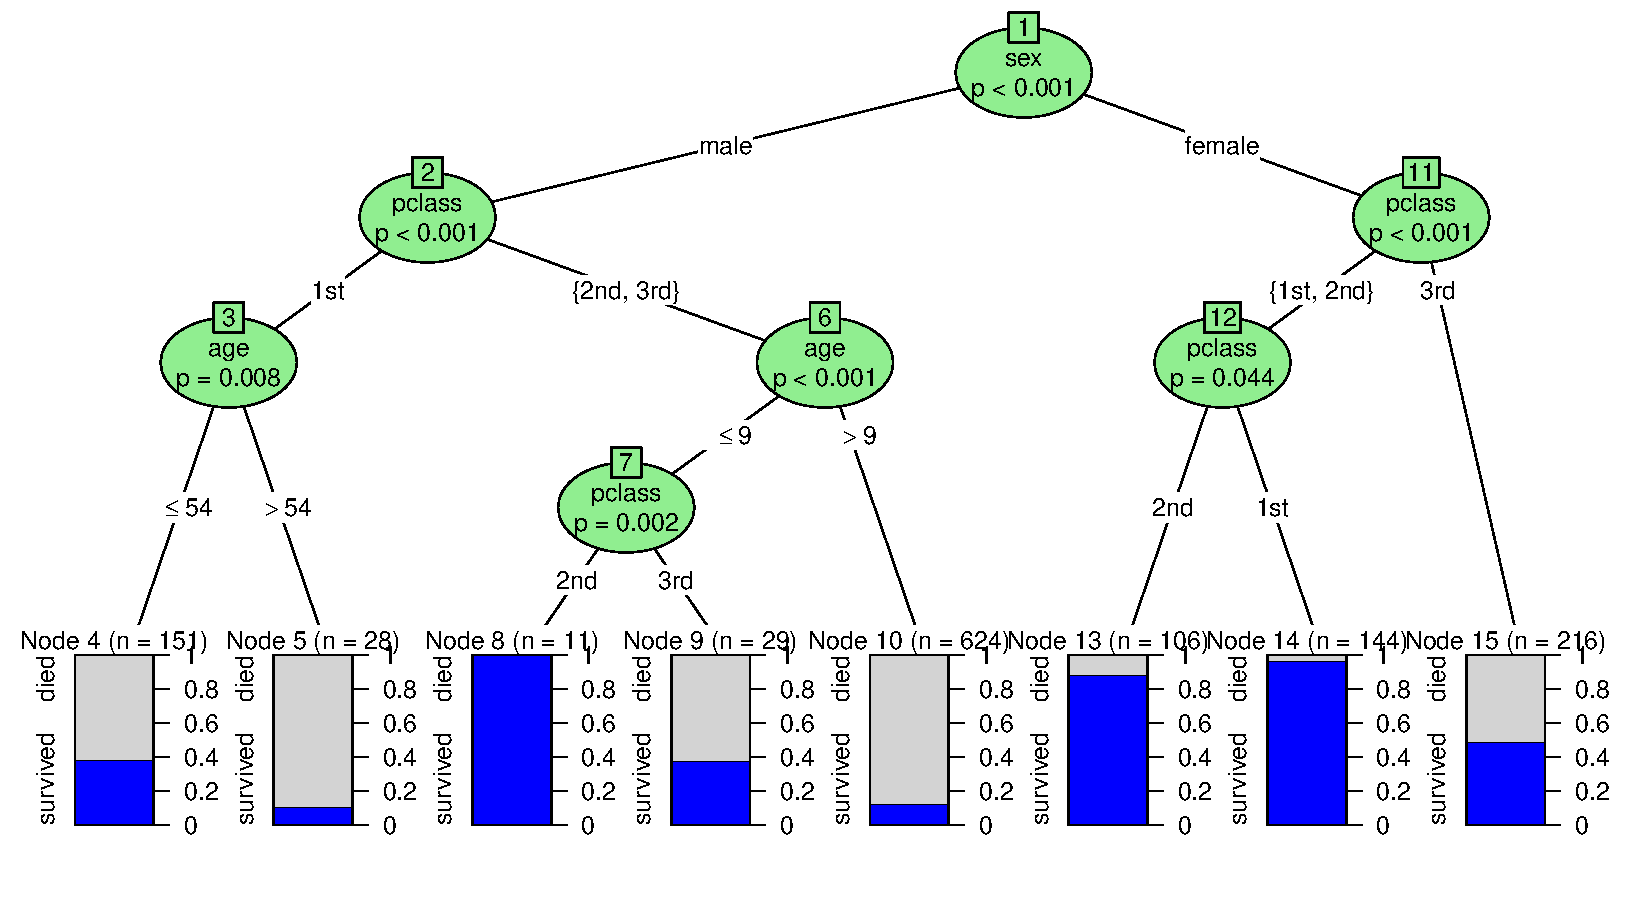
\includegraphics[width=\linewidth]{figure/titanic-ctree-1} 

}

\caption[A conditional inference tree for survival on the Titanic]{A conditional inference tree for survival on the Titanic. The barplots below each leaf node highlight the proportion of survivors in each branch.}\label{fig:titanic-ctree}
\end{figure}


\end{knitrout}
\end{Example}




\bigskip\noindent
\textbf{\R Packages used here}: \textsf{party, strucchange, sandwich, zoo, modeltools, stats4, mvtnorm, grid, plotmo, TeachingDemos, plotrix, rpart.plot, rpart}.


\bibliography{graphics,statistics,ex-packages}
\bibliographystyle{abbrvnat-apa}
\end{document}
